\documentclass[a4paper, 14pt]{extarticle}%тип документа

%Русский язык
\usepackage[T2A]{fontenc} %кодировка
\usepackage[utf8]{inputenc} %кодировка исходного кода
\usepackage[english,russian]{babel} %локализация и переносы

%отступы 
\usepackage[left=2cm,right=2cm,top=2cm,bottom=3cm,bindingoffset=0cm]{geometry}

%Вставка картинок
\usepackage{graphicx}
\usepackage{wrapfig, caption}
\graphicspath{}
\DeclareGraphicsExtensions{.pdf,.png,.jpg, .jpeg}
\newcommand\ECaption[1]{%
     \captionsetup{font=footnotesize}%
     \caption{#1}}

%Таблицы
\usepackage[table,xcdraw]{xcolor}
\usepackage{booktabs}

%Графики
\usepackage{pgfplots}
\pgfplotsset{compat=1.9}

%Математика
\usepackage{amsmath, amsfonts, amssymb, amsthm, mathtools}

%Заголовок
\author{Подлесный Артём \\ группа 827}
\title{Работа 5.1 \\ Измерение коэффициента ослабления потока $\gamma$-лучей и их энергии.}

\begin{document}
\maketitle

\section*{Краткая теория}
Закон ослабления для пучка интенсивности $I_0$:
\begin{equation}
I = I_0 e^{-\mu l}.
\end{equation}
Так как при прохождении через вещество меняется только количество, а не энергия $\gamma$-квантов пучка, то для числа отсчетов получил аналогичную формулу:
\begin{equation}
N = N_0 e^{-\mu l}.
\end{equation}
Отсюда получаем рассчетную формулу для коэффициента ослабления:
\begin{equation}
\mu  = \frac{1}{l} \text{ln}\frac{N_0}{N}.
\end{equation}

\section*{Экспериментальная установка}

Зависимость (2) может невыполняться из-за плохой геометрии, когда рассеянные $\gamma$-кванты остаются в пучке. Для преодоления этого эффекта, во-первых, счинтилляционный счетчик находится на большом расстоянии от поглотителя, а во-вторых, между образцами оставляются промежутки некоторого расстояния, чтобы рассеянные частицы вылетали из потока, и не наблюдалось вторичного комптоновского рассеяния. Схема установки представлена на рис. 1. 

\begin{figure}[h]
\begin{center}
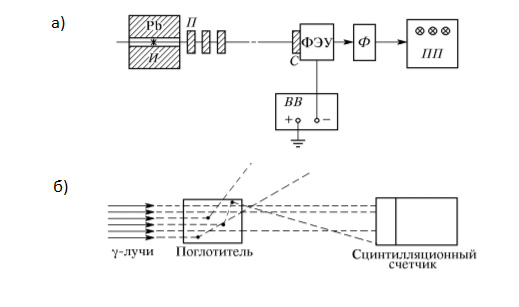
\includegraphics[width=0.9\textwidth]{ust}
\end{center}
\ECaption{a) Схема установки по детекции частиц. \\ б) Схема процесса рассеяния $\gamma$-квантов.}
\end{figure}

\section*{Экспериментальные данные}

В первую очередь был определен фон ($N_{\text{фона}}$) и излучение без поглотителя ($N_0$) за 10 секунд измерений. Источник закрывался свинцовой защитой для измерения фона. Так же в работе был поглотитель из свинцовой трубки, которая значительно толще защиты, однако счетчик показывал тот же результат. Это свидетельствует о надежности свинцовой защиты. Таким образом измеренные значения:
\[ N_{\text{фона}} = 156 \pm 13,\]
\[N_0 = 84433 \pm 174.\]
Далее проводились измерения длин всех участвующих образцов. Эти значения представлены на таблице 1.

\begin{table}[h!]
\begin{center}
\begin{tabular}{|c|c|c|c|}
\hline
\rowcolor[HTML]{9698ED} 
№  & Алюминий, мм & Железо, мм & Свинец, мм \\ \hline
1 & 20       & 10     & 5      \\ \hline
\rowcolor[HTML]{9698ED} 
2 & 20       & 10     & 4.5    \\ \hline
3 & 19.8     & 10     & 4.6    \\ \hline
\rowcolor[HTML]{9698ED} 
4 & 20       & 10     & 4.9    \\ \hline
5 & 20.3     & 10.3   & 4.9    \\ \hline
\end{tabular}
\ECaption{Точность измерений длин поглотителей составляет 0.1 мм. Поглотители имеют свой номер, который соответствует порядку их добавления в экспериментальную установку.}
\end{center}
\end{table}

Каждый из этих образцов добавлялся согласно своему порядковому номеру в установку, то есть в эксперименте с железом №2 присутствовали поглотители из железа с номерами 1 и 2. Все поглотители находились на примерно одинаковом расстоянии друг от друга. Результаты эксперимента на таблице 2.
\newpage

\begin{table}[h!]
\begin{center}
\begin{tabular}{|c|c|c|c|c|c|}
\hline
\rowcolor[HTML]{9698ED} 
железо   & 1     & 2     & 3     & $N_{\text{среднее}}-N_{\text{фона}}$ & $\sigma_{\text{среднего}}$ \\ \hline
1        & 47213 & 47723 & 47282 & 47250                                & 160                        \\ \hline
\rowcolor[HTML]{CBCEFB} 
2        & 26546 & 27016 & 26951 & 26682                                & 147                        \\ \hline
3        & 15153 & 15446 & 15479 & 15203                                & 104                        \\ \hline
\rowcolor[HTML]{CBCEFB} 
4        & 8912  & 8828  & 8745  & 8672                                 & 48                         \\ \hline
5        & 5075  & 4947  & 5122  & 4892                                 & 52                         \\ \hline
\rowcolor[HTML]{9698ED} 
свинец   & 1     & 2     & 3     & $N_{\text{среднее}}-N_{\text{фона}}$ & $\sigma_{\text{среднего}}$ \\ \hline
1        & 46309 & 46168 & 46423 & 46144                                & 74                         \\ \hline
\rowcolor[HTML]{CBCEFB} 
2        & 27878 & 27569 & 27627 & 27535                                & 95                         \\ \hline
3        & 17012 & 16603 & 16675 & 16607                                & 126                        \\ \hline
\rowcolor[HTML]{CBCEFB} 
4        & 9719  & 9996  & 9646  & 9631                                 & 107                        \\ \hline
5        & 5882  & 6022  & 5990  & 5809                                 & 42                         \\ \hline
\rowcolor[HTML]{9698ED} 
алюминий & 1     & 2     & 3     & $N_{\text{среднее}}-N_{\text{фона}}$ & $\sigma_{\text{среднего}}$ \\ \hline
1        & 56037 & 55988 & 55968 & 55842                                & 20                         \\ \hline
\rowcolor[HTML]{CBCEFB} 
2        & 37098 & 37025 & 37070 & 36908                                & 21                         \\ \hline
3        & 24367 & 24547 & 24754 & 24400                                & 112                        \\ \hline
\rowcolor[HTML]{CBCEFB} 
4        & 16365 & 16526 & 16307 & 16243                                & 66                         \\ \hline
5        & 11203 & 11189 & 11116 & 11013                                & 27                         \\ \hline
\end{tabular}
\ECaption{Результаты измерений ослабления потока частиц. По горизонтали для каждого материала -- кол-во поглотителей, по вертикали -- номер измерения. Каждый эксперимент повторялся 3 раза. }
\end{center}
\end{table}

Исходя из этих данных возможно построить график ослабления для каждого материала. Исходя из (3) получим линейную зависимость 
\begin{equation}
 \text{ln}\frac{N_0}{N}=\mu l.
\end{equation}
Она представлена на рис 2.

\begin{figure}[h!]
\begin{center}
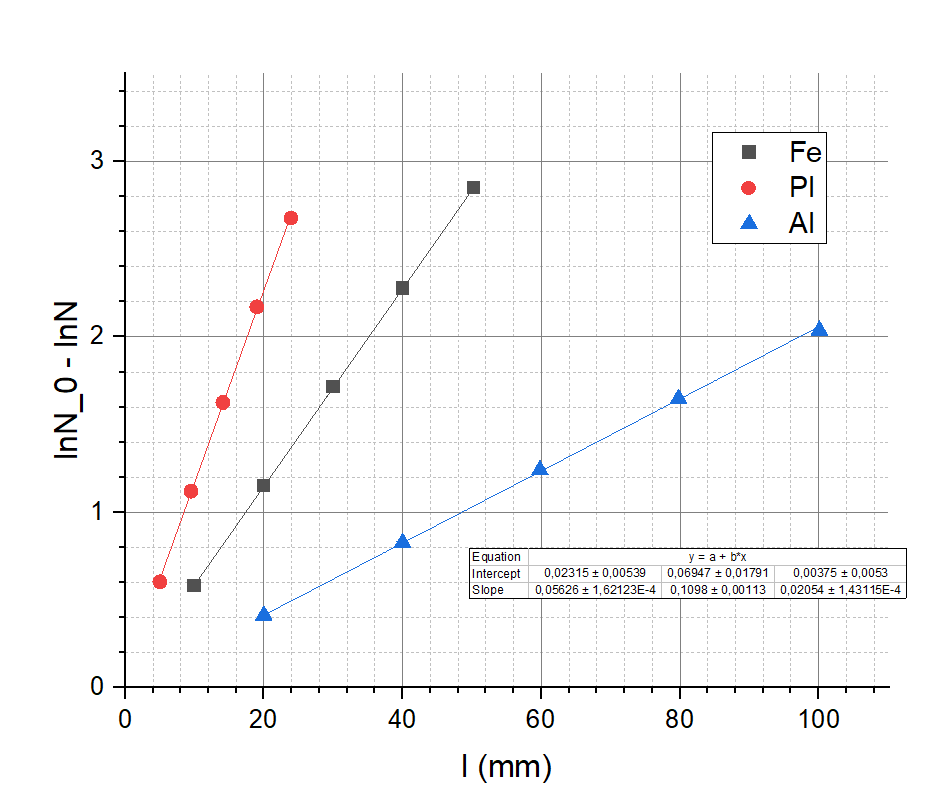
\includegraphics[width=0.9\textwidth]{gr}
\end{center}
\ECaption{График зависимости $ln\frac{N_0}{N}(l)$. Каждая прямая подписана своим материалом. Как видно, данные предоставлены с хорошей точностью.}
\end{figure}

Отсюда получим искомые значения коэффициента ослабления каждого материала, как угол наклона прямой. Исходя из теоретической зависимости коэффициента ослабления, так же определяем среднюю энергию $\gamma$-квантов в нашем эксперименте. Результаты представлены на таблице 3.

\begin{table}[h!]
\begin{center}
\begin{tabular}{|c|c|c|c|}
\hline
\rowcolor[HTML]{9698ED} 
         & $\mu$, cм$^{-1}$ & $\sigma_{\mu}$, cм$^{-1}$ & $E_{\gamma}$, МэВ \\ \hline
Железо   & 0.563            & 0.002                     & 0.7               \\ \hline
\rowcolor[HTML]{9698ED} 
Алюминий & 0.205            & 0.002                     & 0.65              \\ \hline
Свинец   & 1.1              & 0.01                      & 0.7               \\ \hline
\end{tabular}
\ECaption{Результаты измерений. Примерное значение для энергии квантов.}
\end{center}
\end{table}
\newpage
\section*{Вывод}
Показано, что закон ослабления $\gamma$-квантов выполняется достаточно точно. Так как экспериментально определенные значения коэффициентов ослабления поглотителей соответствуют примерно одному значению энергии, а параметры установки не менялись на протяжении эксперимента, то можно говорить о достаточной достоверности результатов.

















































\end{document}